 \section{Evaluation}
 \label{sec:eval}

 In our comprehensive assessment of \Sys, we explore several key research questions. Our testing environment comprised a machine with 8 Intel vCPUs, 80 GB RAM, an NVIDIA RTX2080 GPU, and ran on Ubuntu 18.04.6 LTS.
\wajih{you need add results related to resource overheads, hyperparameters tuning, ablation study, etc. Almost all the experiments that you have in your Flash paper are also applicable here.}

\wajih{please add all the research questions here even if you are still running the experiments.}

\begin{itemize}[leftmargin=*]
\item \textbf{RQ1.} What is the comparative detection accuracy of \Sys against current systems?
\item \textbf{RQ2.} What is the effectiveness of word2vec harmonization in a utility server setting?
\end{itemize}

\PP{Implementation} We developed \Sys using Python and incorporated the Torch Geometric library for our \gnnshort model. This model employs Sage Convolutions, a graph convolution layer that aggregates features from adjacent nodes to generate new node features. To enhance generalization, the model integrates dropout and ReLU activation functions across layers. For our \wordvec model, we utilized the Gensim library.

\PP{Datasets} \Sys underwent testing with two open-source datasets: \darpa E3~\cite{darpae3} and \darpa \optc~\cite{darpatc}. The E3 dataset, originating from \darpa's third red-vs-blue team exercise, includes audit logs depicting both normal and malicious activities. The \darpa \optc dataset offers a comprehensive view of benign and malevolent audit records from around 1000 hosts. It features six days of normal activities for training, followed by three days showcasing different types of attacks for evaluation purposes. The first day simulates a PowerShell Empire staging scenario, including the initial breach, lateral movements, and privilege escalations. The second day focuses on data exfiltration events, while the third day involves the deployment of malicious software.

\PP{Detectors for Comparison} For benchmarking \Sys, we employed the \threatrace \cite{wang2022threatrace} system, adopting the same detection metrics for comparison. \threatrace, a provenance-based IDS, leverages a \gnn for node-level anomaly detection. It learns the structural patterns of nodes in benign datasets and detects anomalies based on deviations from these patterns. Unlike \Sys, however, \threatrace does not ensure the privacy of user logs and faces scalability issues.

{\renewcommand{\arraystretch}{1.2}% for the vertical padding
\begin{table*}[t!]
  \centering
  \scriptsize
  \caption{Comparison of \Sys against FLASH and KAIROS. Prec.: Precision; Rec.: Recall;}
  \setlength{\tabcolsep}{0.7pt}
  \begin{tabular}{ccccccccccccc}
    \toprule

  \multirow{2}{*}{\textbf{Datasets}}
  & \multicolumn{4}{c }{\Norothead{ \bf \Sys}}
  & \multicolumn{4}{c }{\Norothead{ \bf FlASH}}
  & \multicolumn{4}{c }{\Norothead{ \bf KAIROS}}
  \\ \cmidrule(r{\tbspace}){2-5} \cmidrule(r{\tbspace}){6-9} \cmidrule(r{\tbspace}){10-13}

    & {\bf Prec.} &  {\bf Rec.} & {\bf \fscore} & {\bf TP}/ {\bf FP}/ {\bf FN}/ {\bf TN} & {\bf Prec.}  & {\bf Rec.} & {\bf \fscore} & {\bf TP}/ {\bf FP}/ {\bf FN}/ {\bf TN} & {\bf Prec.}  & {\bf Rec.} & {\bf \fscore} & {\bf TP}/ {\bf FP}/ {\bf FN}/ {\bf TN} \\

  \midrule

  E3-CADETS &  0.90 & 0.99 & 0.95 & 12846/ 1408/ 6/ 705,558 & 0.94 & 0.99 & 0.96 & 12851/ 818/ 1/ 706,148 & 0.80 & 1.00 & - & 4/ 1/ 0/ 174 \\
  E3-TRACE &  0.95 & 0.99 & 0.97 & 67357/ 3161/ 26/ 2,412,846 & 0.95 & 0.99 & 0.97 &  67382/ 3477/ 1/ 2,412,530 & - & - & - & - \\
  E3-THEIA &  0.89 & 0.99 & 0.94 & 25311/ 3155/ 51/ 3,502,171 & 0.92 & 0.99 & 0.95 & 25318/ 2282/ 44/ 3,503,044 & 0.67 & 1.00 & - & 10/ 1/ 0/ 216 \\  
  OpTC & 0.88 & 0.94 & 0.91 & 610/ 80/ 40/ 1,287,275 & 0.93 & 0.92 & 0.93 & 600/ 43/ 50/ 1,287,312 & 0.84 & 1.00 & - & 32/ 6/ 0/ 1210 \\
  \bottomrule
  \end{tabular}
\label{summary:benchmarks:large}
\end{table*}}

 \subsection*{RQ1. Detection Performance}
 Table~\ref{summary:benchmarks:large} presents a comparative analysis of the detection performance between \Sys and \threatrace. It reveals that \Sys achieves a detection performance comparable to that of \threatrace. The advantage of \Sys lies in its ability to preserve user log privacy via federated learning. Additionally, its scalability is enhanced as each client independently conducts anomaly detection on their logs. This decentralization of learning and detection tasks, enabled by federated learning, significantly enhances the scalability of our system.

 \subsection*{RQ2. Efficacy of Word2vec harmonization}
 To evaluate the efficacy of our method, we performed experiments comparing the utility server-based harmonized model with a local word2vec model on each client. These experiments utilized the \optc dataset. The findings, detailed in Table~\ref{local:wordvec}, demonstrate that our strategy significantly enhances the performance of \Sys. This improvement is attributed to our approach's ability to minimize noise in disparate word2vec vectors, thereby facilitating a more accurate interpretation of various activity patterns in the provenance graph by the \gnnshort model.

\begin{table}[h!]
    \centering
    \scriptsize
      \caption{Effectiveness of word2vec vectors harmonization.}
        \begin{tabular}{ | c | c | c | c | c | c |}
          \hline
            \bf Word2vec Type & \bf Precision & \bf Recall & \bf \fscore & \bf TP & \bf FP \\
          \hline
           Vanilla & 0.66  & 0.97 & 0.79 & 636 & 325 \\
           Harmonized & 0.88 & 0.94 & 0.91 & 610 & 80 \\
          \hline
        \end{tabular}
        \label{local:wordvec}
    \end{table}

\subsection*{Effect of Hosts vs Detection Performance}

\begin{figure}[t!]
  \centering
  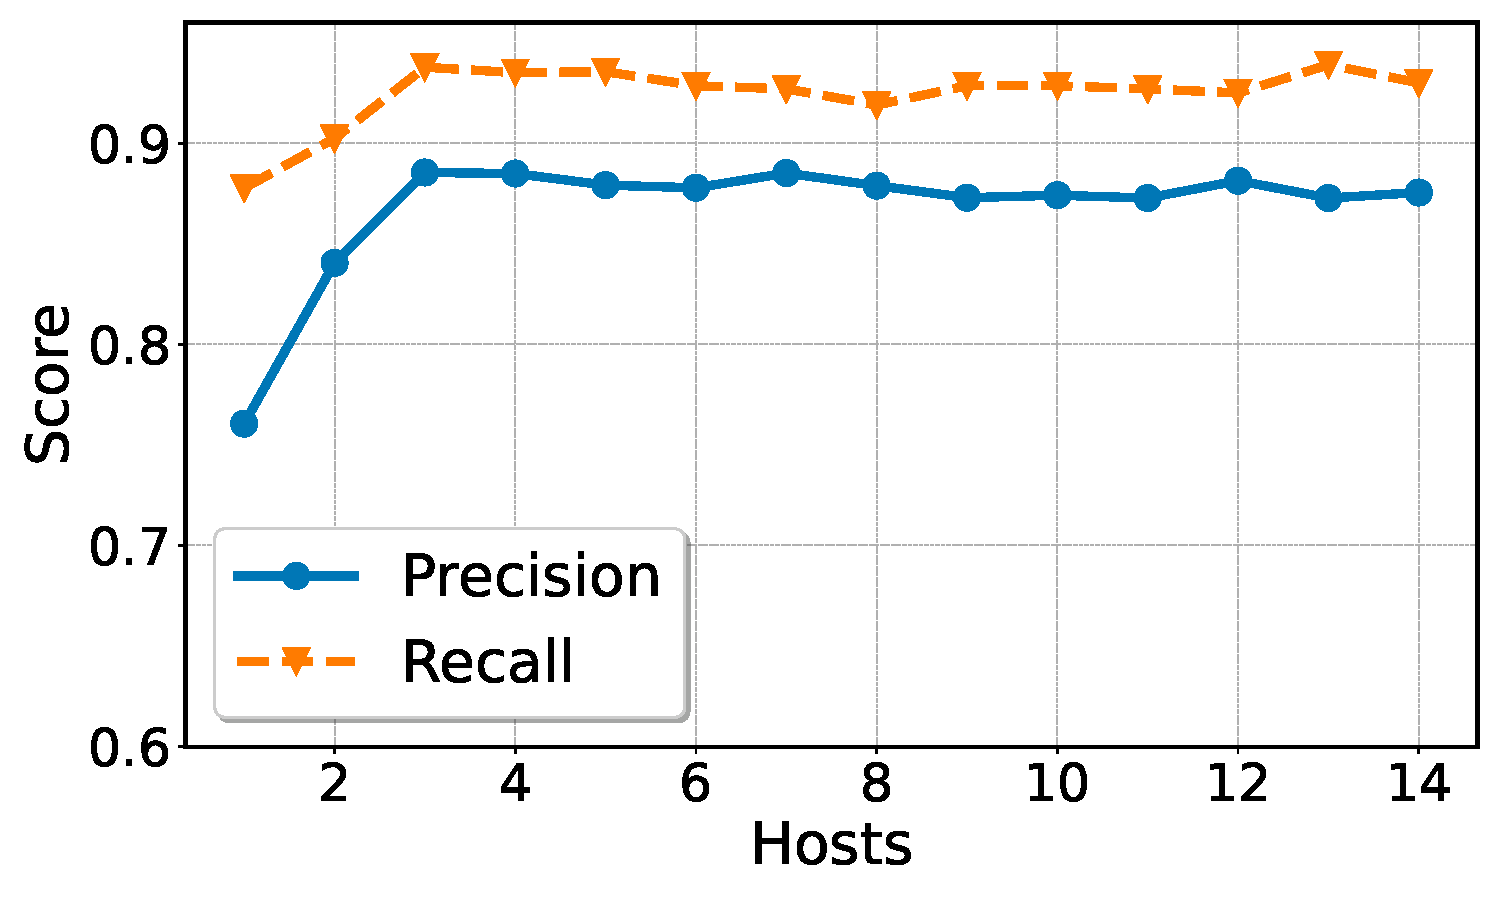
\includegraphics[width=0.50\textwidth]{fig/scoresvshosts.pdf}
  \caption{Effect of number of hosts vs detection metrics.}
  \label{scoresvshosts}
  \vspace{-2ex}
\end{figure}

\begin{figure}[t!]
  \centering
  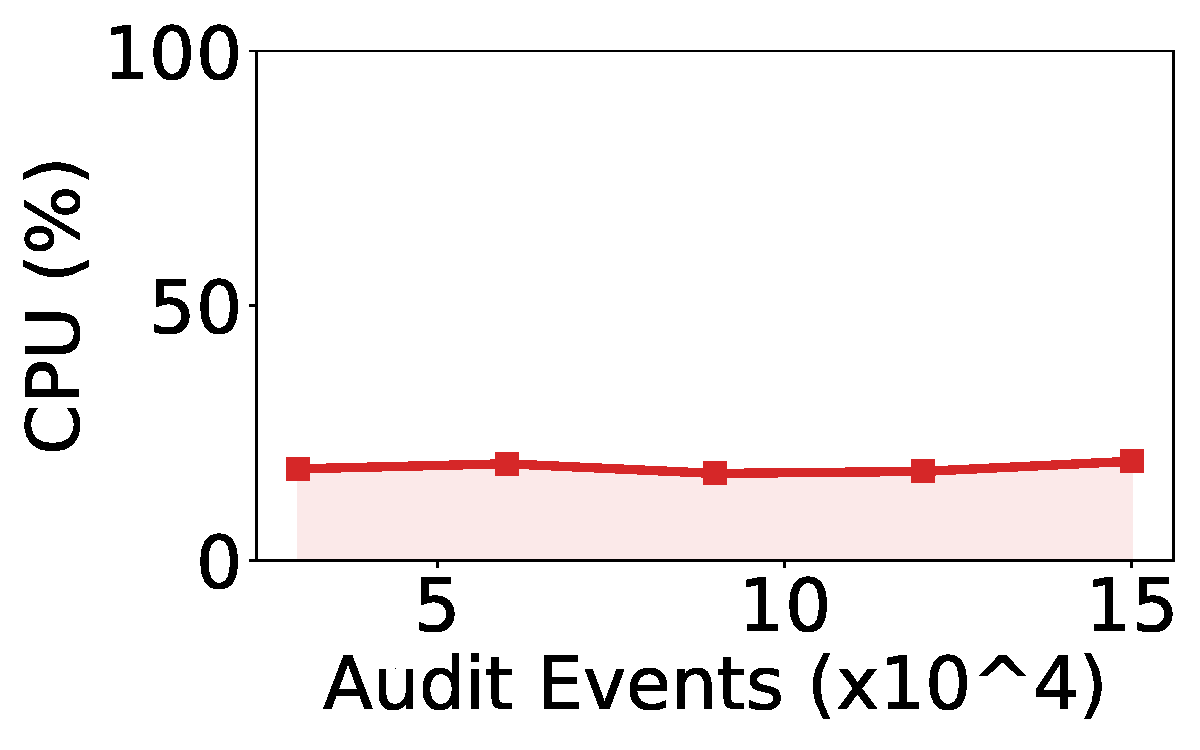
\includegraphics[width=0.50\textwidth]{fig/cpu.pdf}
  \caption{CPU Usage}
  \label{cpu}
  \vspace{-2ex}
\end{figure}

\begin{figure}[t!]
  \centering
  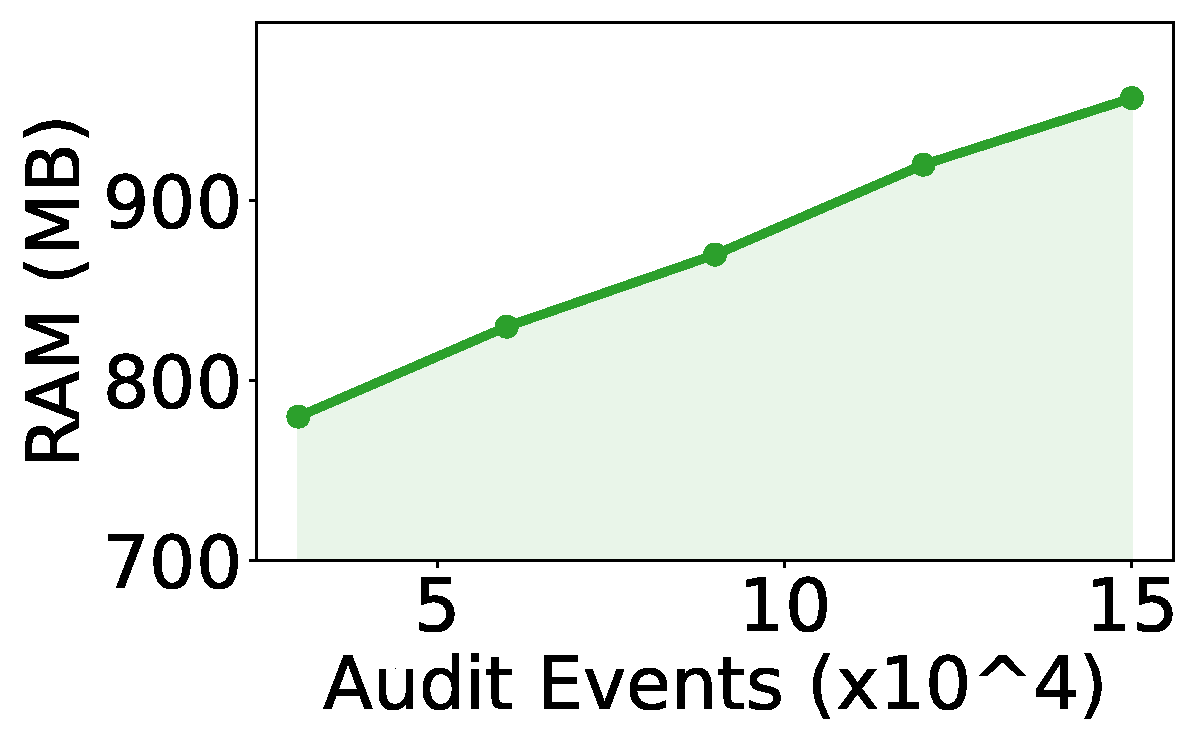
\includegraphics[width=0.50\textwidth]{fig/ram.pdf}
  \caption{RAM usage}
  \label{ram}
  \vspace{-2ex}
\end{figure}

\begin{figure}[t!]
  \centering
  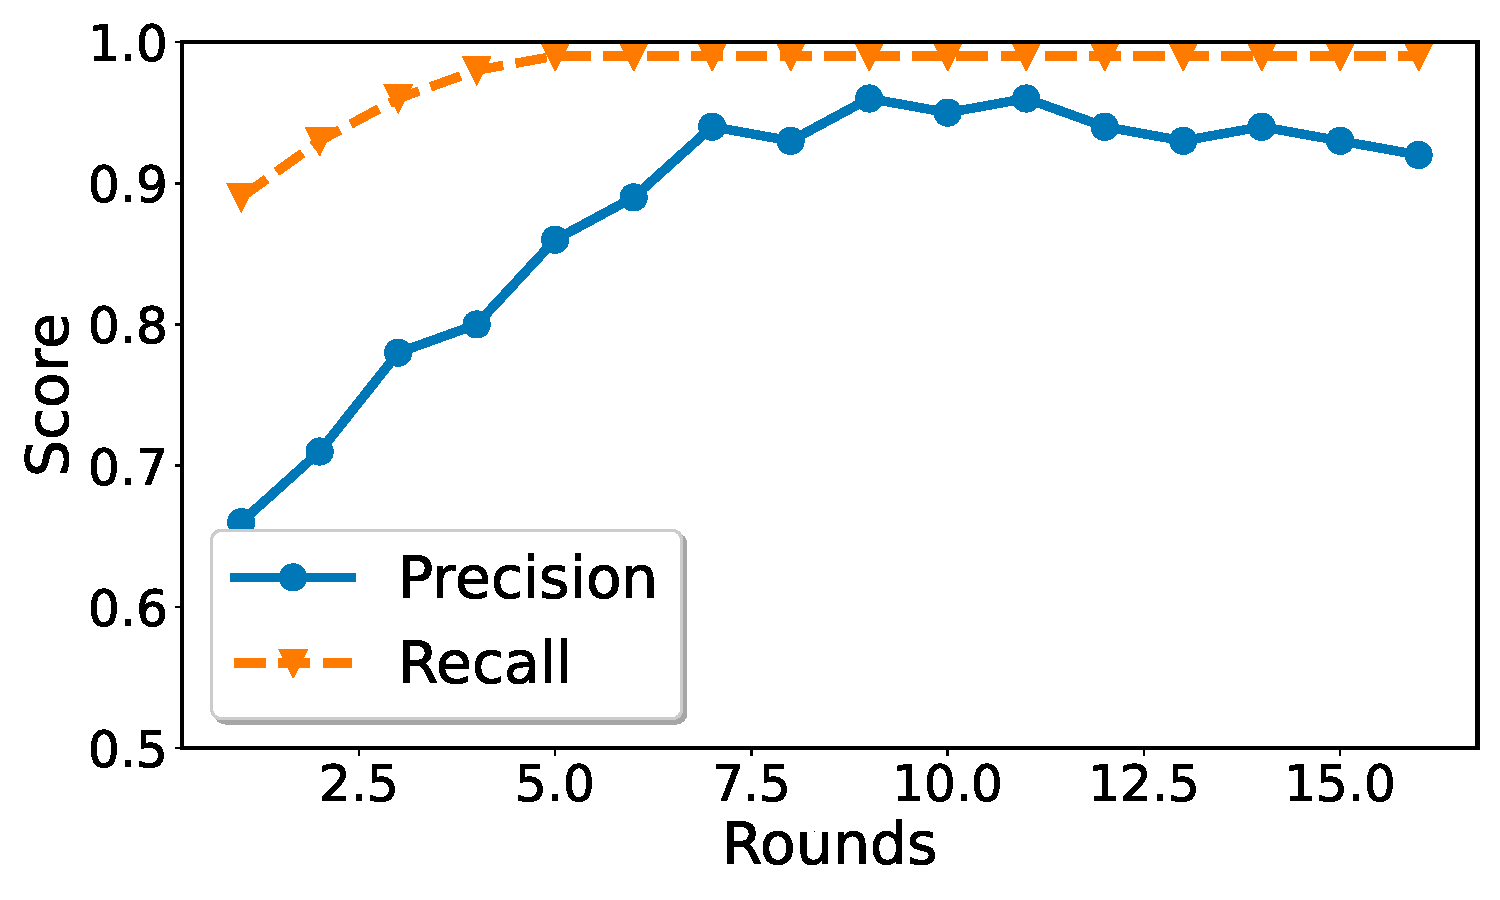
\includegraphics[width=0.50\textwidth]{fig/roundsvsscore.pdf}
  \caption{Federated Averaging Rounds vs Detection Performance.}
  \label{roundsvsscore}
  \vspace{-2ex}
\end{figure}

\begin{figure}[t!]
  \centering
  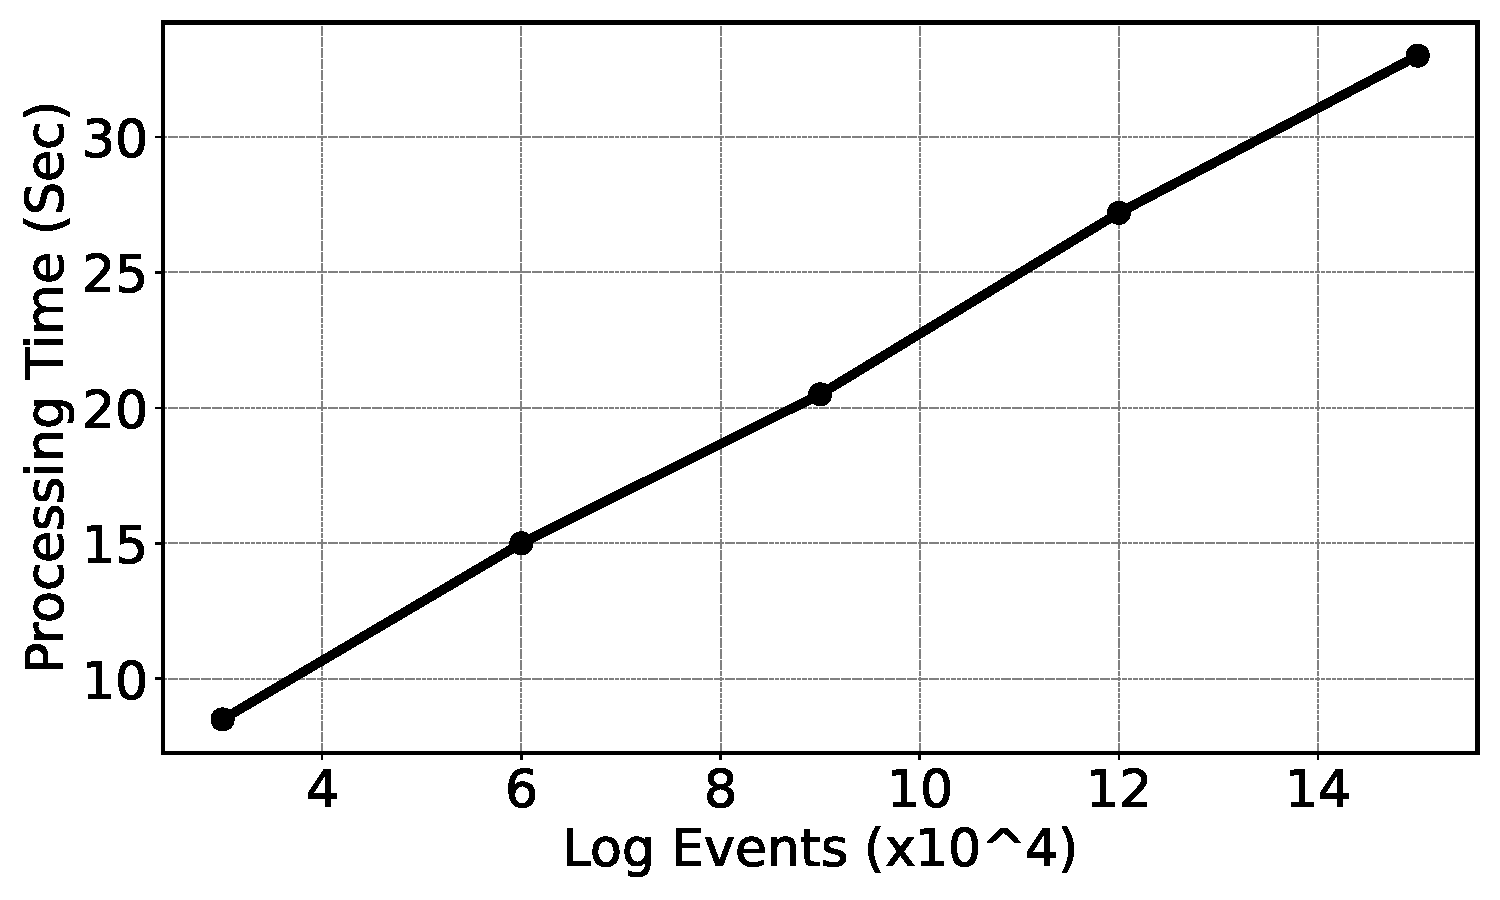
\includegraphics[width=0.50\textwidth]{fig/sizevstime.pdf}
  \caption{Processing Time for various Audit Event Sizes}
  \label{sizevstime}
  \vspace{-2ex}
\end{figure}

\begin{figure}[t!]
  \centering
  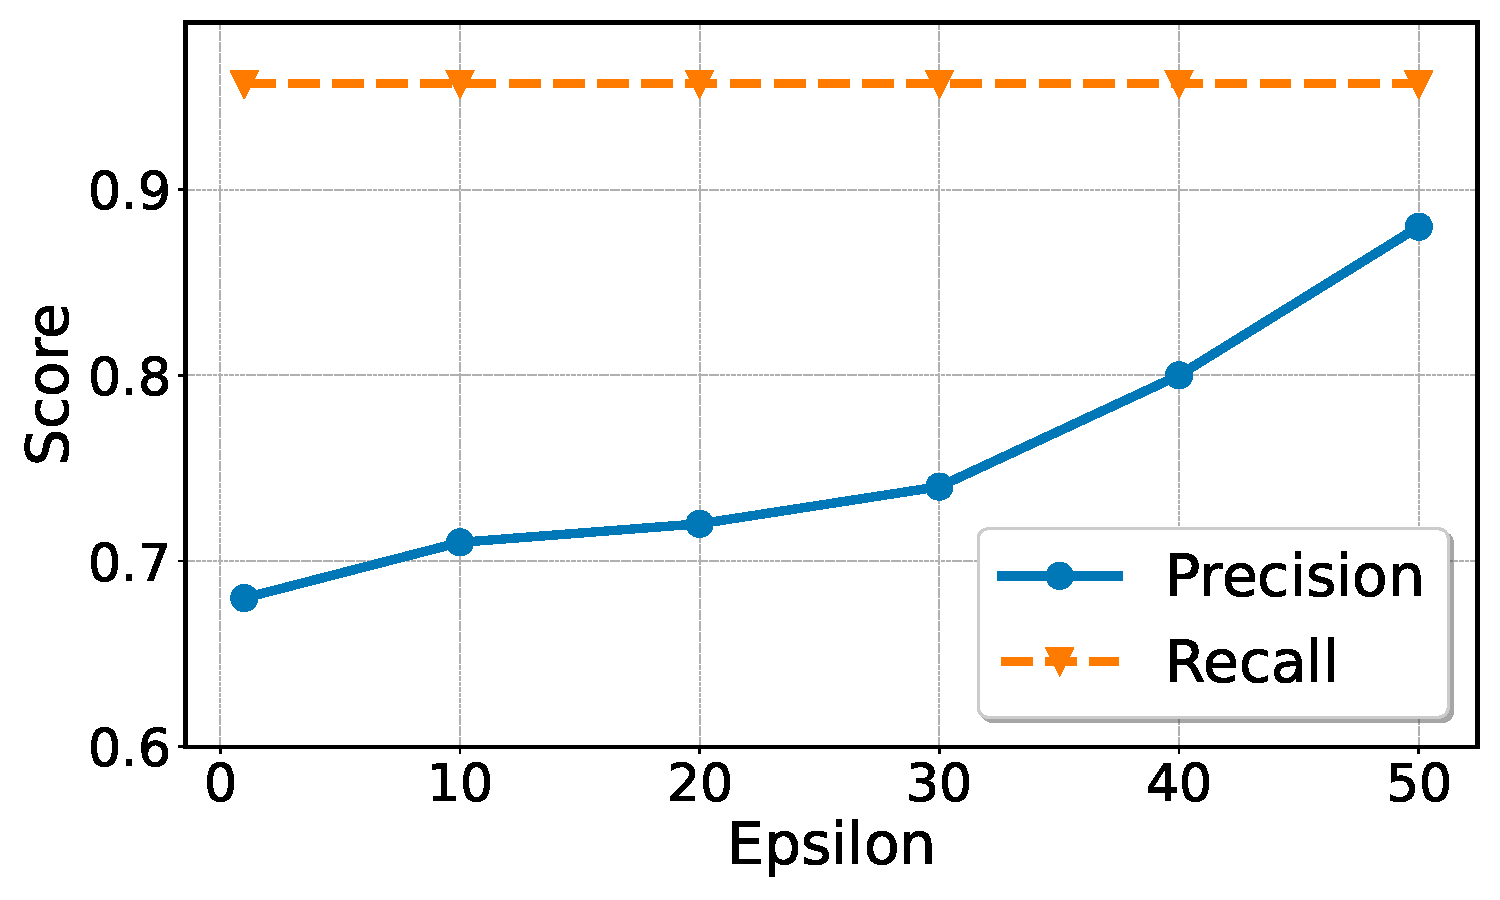
\includegraphics[width=0.50\textwidth]{fig/epsvsscore.pdf}
  \caption{Effect of Different LDP Noise Level on Detection Performance.}
  \label{epsvsscore}
  \vspace{-2ex}
\end{figure}

\subsection*{CPU and Resource consumption}

